\section{Experimental Evaluation}\label{sec:experiments}
We now describe the experiments to be conducted for this study.
The goals for the experiments are to answer the following questions w.r.t two strategies namely pipelining (PIPE) and non-pipelining (NPIPE):
\begin{enumerate}
	\item Which strategy results in a better response time for a query under various scenarios?
	\item Why does the better strategy outperform the other strategy?
\end{enumerate}

We conduct our experiments in \sys{}, an in-memory database engine. 
We describe the proposed methodology below. 

\subsection{Workload}
We use queries and dataset from the TPC-H benchmark~\cite{tpc-h} for scale factor 50.

We perform an analysis of the TPC-H queries based on how they are impacted by pipelining. 
Note that the analysis uses query plans generated by \sys{}'s cost based query optimizer. 

We acknowledge that systems may differ based on their cost models, heuristics and general query optimization techniques.
Moreover \sys{} uses hash based implementation of join algorithms, which makes a pipeline of (selection operator $\rightarrow$ probe operator) possible. 
Other systems may use different join algorithm that may not have possibility of pipelining. 
Therefore the suitability of queries for pipelining analysis for \sys{} may not be the same for other systems.
However the principles that we use to determine the suitability of a query for pipelining study should be broadly applicable for different systems as well as workloads other than TPC-H. 

\begin{figure}
	\centering 
	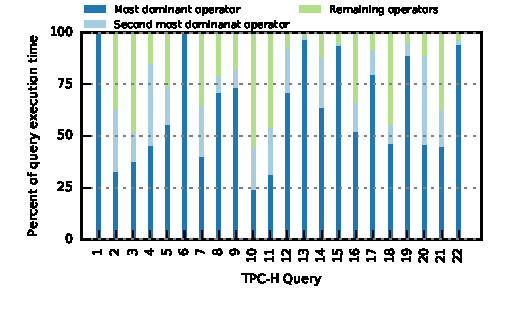
\includegraphics[width=0.65\textheight]{pipeline/figures/all-tpch-queries-time-distribution}
	\caption{Distribution of time spent in each TPC-H query among its operators.}
	\label{fig:time-distribution-all-tpch}
\end{figure}

We describe those principles in the next section.
The suitability of the queries is presented in Table~\ref{table:pipelining-suitability-tpch}.

\subsection{Suitability of TPC-H queries for pipelining study}
To determine whether a query is suitable for the pipelining study or not, we study the time spent in individual operators.
The intuition is that if there is only one operator in the query where majority of the query execution time is spent, pipelining may not play a big role in the overall execution time of the query.
To make the analysis simpler, we analyze the most dominant operator (where the highest time is spent) and the second most dominant operator. 
Note that for this analysis, we run the queries in the non-pipelining mode, so that the percent time spent metric is accurate.

Figure~\ref{fig:time-distribution-all-tpch} shows the results of this experiment. 
For some queries (Q1, Q6, Q13, Q15, Q17, Q19, Q22) the dominant operator takes up the majority of the query execution time, and thus make them unsuitable for our analysis.
We make an exception for Q19, as it is a simple query with one join and selections on the build and probe side.
Thus it is easy to analyze the impact of pipelining on this query.

In many queries even though there are pipelines of operators, majority of the data is pruned out at the base of the pipeline. 
Therefore not enough data is passed on to the consumer operators and hence the impact of pipelining is minimal. 
Hence we do not consider such queries for our study (Q11, Q12, Q17 \todo{verify}).

A good candidate for our pipeline study is a query that has a large input to the pipeline and has significant amount of data gets passed through the pipeline. 

\begin{table}[]
	\centering
	\begin{tabular}{|p{1.1cm}|p{14cm}|c|}
		\hline
		\textbf{Query} & \textbf{Comment} & \textbf{Suitable?} \\ \hline
		1 & Single operator, no scope for pipelining & No \\ \hline
		2 & Big hash join probe $\rightarrow$ aggregate pipeline & Yes \\ \hline
		3 & Big selection $\rightarrow$ probe join hash table $\rightarrow$ aggregate pipeline & Yes \\ \hline
		4 & Two pipelines, both with large inputs & Yes \\ \hline
		5 & Two pipelines involving probe operators & Yes \\ \hline
		6 & Single operator, no scope for pipelining & No \\ \hline
		7 & One big pipeline consisting of selection, hash join probes and aggregation & Yes \\ \hline
		8 & Multiple pipelines made up of selections, building and probing join hash tables, and aggregation & Yes \\ \hline
		9 & Single pipeline made up of hash join probes and aggregation & Yes \\ \hline
		10 & Multiple pipelines made up of selections, building and probing join hash tables, and aggregation & Yes \\ \hline
		11 & Small query execution time & No \\ \hline
		12 & One pipeline with little work at the end of the pipeline & No \\ \hline
		13 & No pipeline has enough work & No \\ \hline
		14 & One pipeline with selection, probing join hash table and aggregation & Yes \\ \hline
		15 & No pipeline has enough work & No \\ \hline
		16 & Majority of time is spent in an operator at the end of a pipeline & No \\ \hline
		17 & Majority of work is in the aggregation which is the leaf level operator in the query plan DAG & No \\ \hline
		18 & Dominant operator is not part of a pipeline & No \\ \hline
		19 & Single pipeline of selection and probing of join hash table & Yes \\ \hline
		20 & Two dominant operators are connected by a pipelining breaking edge & No \\ \hline
		21 & \todo{Redo} & Yes \\ \hline
		22 & Most dominant operator is build hash operator. & No \\ \hline
	\end{tabular}
	\caption{Analysis of TPC-H queries to determine their suitability for the pipelining study}
	\label{table:pipelining-suitability-tpch}
\end{table}

To compare the two strategies, we measure each query's response time under each strategy.
In some cases we measure hardware counters such as L3 cache miss ratio.

\subsection{Storage Format}
To explore the relationship between pipelining performance and storage formats, we use two storage formats for our evaluation namely row store and column store.
All the base tables in the TPC-H schema are stored in the same storage format.
We use row store format for temporary tables irrespective of the storage format of the base tables.

Column stores have shown to have higher performance for analytical workloads~\cite{AbadiMH08}. 
However recent studies~\cite{quickstep-vldb} have shown that the performance gap between column stores and row stores is not as high as shown earlier.
Therefore we use both storage formats for our comparison. 

\subsection{Block Size}
We start by explaning the concept of block size.
As the producer operator processes the input, it materializes the output to a temporary block. 
We let the temporary block to reach a threshold size (known as block size) and then pass the block to the consumer operator. 

We would like to examine the impact of block size on the performance of the pipelining strategies. 
Consider an example pipeline: select operator $\rightarrow$ probe hash table operator.
A smaller block size in the pipelining strategy would mean that the block can potentially get filled quickly. 
Therefore, compared to a larger block size, the probe tasks may be scheduled more frequently and each task itself may be shorter. 

\subsection{Hardware Description}
We now describe the hardware configuration and \sys{} specifications used for our evaluation. 
The hardware configuration of the machine that we used are described in Table~\ref{table:pipeline-hardware}.

\begin{table}[h]
	\centering
	\begin{tabular}{|c|c|}
		\hline
		\textbf{Parameter} & \textbf{Description} \\ \hline
		Processor & 2 Intel Xeon Intel E5-2660 v3 2.60 GHz (Haswell EP) processors\\ \hline
		Cores & 10 physical, 20 with hyper-threading per socket \\ \hline
		Memory & 80 GB per NUMA socket, 160 GB total \\ \hline
		Caches & L3: 25 MB, L2: 256 KB, L1 (both instruction and data): 32 KB \\ \hline
		OS & Ubuntu 14.04.1 LTS \\ \hline
	\end{tabular}
	\caption{Evaluation platform}
	\label{table:pipeline-hardware}
\end{table}

The focus of our study is on a single NUMA socket, therefore we only use Socket 0 for our experiments. 
Unless specified, we use all the 20 threads on socket 0.
\sys{} is configured with all 20 threads to be used as worker threads.
It uses 80\% of the system's memory as the buffer pool size (126 GB).
We run each query 5 times and report the mean of the three best runs. 
We perform hardware instrumentation using Processor Counter Monitor (PCM) library~\cite{pcm}.

\subsection{Results}
In this section we discuss the results of our experimental evaluation. 
We report two metrics: Overall query response time and mean execution time of operator (Select and Probe) tasks.
As we are interested in the relative performance of non-pipelining implementation and pipelining implementation, we plot the relative improvement of one strategy over other. 

\begin{figure}
	\centering 
	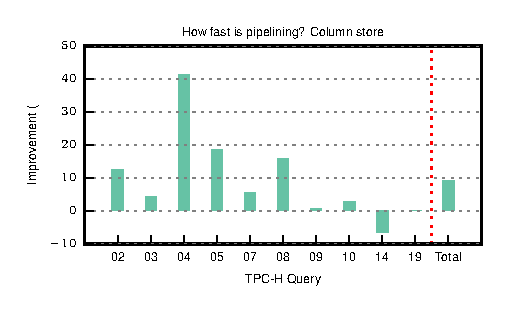
\includegraphics[width=0.6\textheight]{pipeline/figures/bs2mb-20threads-colstore-total-time}
	\caption{Performance comparison of pipelining strategy and non-pipelining strategy using 20 threads, column store storage format and block size of 2 MB.}
	\label{fig:bs2mb-20threads-colstore-total-time}
\end{figure}

\subsubsection{Overall Execution Time:}\label{ssec:overall-execution-time} We first compare the overall execution time of queries using pipelining and non-pipelining strategies. 
We use column store storage format for base and temporary tables and all blocks are sized to 2 MB.
Figure~\ref{fig:bs2mb-20threads-colstore-total-time} presents \% improvement of pipelining strategy over non-pipelining strategy.
In terms of total time, both strategies perform nearly equal. 
This is a surprising observation that pipelining and non-pipelining are not that far off in terms of overall performance. 
However for some queries, non-pipelining is significantly slower (e.g. Q04, 40\%). 

\begin{figure}
	\centering 
	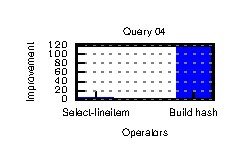
\includegraphics[width=0.3\textheight]{pipeline/figures/tpch-q04-ccs-20threads-bs2mb-meanwo}
	\caption{Comparison of mean work order execution times for TPC-H Q04 in the non-pipelining vs pipelining strategies}
	\label{fig:tpch-q04-ccs-meanwo}
\end{figure}

We then dig deep to find out the why pipelining strategy outperforms non-pipelining for TPC-H Q04. 
We analyze the query execution profile for Q04 in the non-pipelining strategy and find that majority of time (more than 80\%) is spent in a two operator pipeline: The producer is a selection operator whose input is lineitem table and a build hash table operator which is the consumer. 
Note that typically lineitem, which is the largest table in the TPC-H schema is on the probe side. 
However for Q04, \sys{}'s optimizer determines that lineitem should be on the build side.  

Figure~\ref{fig:tpch-q04-ccs-meanwo} compares the performance of the two operators mentioned above.
Notice that the selection operation has similar performance in both cases. 
However the build operation is significantly faster (close to 120\%) in the pipelining case.
The reason for its faster performance is that the effective concurrency of the build hash operator is lower in the pipelining case.
In \sys{}, the build operator's performance does not scale linearly with increasing the degree of parallelism. 
In the non-pipelining strategy, the build hash operator uses all the 20 threads.

Also notice that the gains for the build hash operator in pipelining strategy (120\%) reduce significantly when comparing to the gains of the overall query execution time (40\%). 
This is a salient conclusion that though pipelining is important and useful for getting good performance; its
benefits in the overall query execution time could be suppressed by performance of other operators that are unaffected by pipelining.

\begin{figure}
	\centering 
	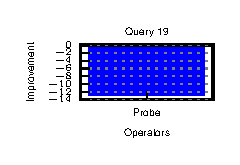
\includegraphics[width=0.4\textheight]{pipeline/figures/tpch-q19-ccs-20threads-bs2mb-meanwo}
	\caption{Comparison of mean work order execution times for TPC-H Q19 in the non-pipelining vs pipelining strategies}
	\label{fig:tpch-q19-ccs-meanwo}
\end{figure}

We pick another query TPC-H Q19 whose performance is nearly same in the non-pipelining and pipelining strategies. 
There is a single pipeline consisting of a selection operation on lineitem table and a hash join probe operator.
Figure~\ref{fig:tpch-q19-ccs-meanwo} compares the performance of these two operators using the two strategies.
The selection operator's performance is nearly identical in both strategies, however the probe operator's performance is slighly poor in the pipelining case. 
As there is no substantial difference between the performance of dominant operators, the overall query execution time is identical in both strategies.

We suspect the slight drop in probe performance of probe operator is due to the small size of the join hash table (\todo{what is the size?}). 
In the non-pipelining case, the hash table is probed more frequently and thus could be resident in L3 cache. 
In the pipelining case, it gets probed less frequently and thus there is less chance that it would be L3 cache resident. 

\subsubsection{Effect of block size:}
We set out to examine the effect of block size on the pipelining performance. 
In each experiment, we set the block size of the base tables and temporary tables to a given value. 
We experiment with two block sizes 1 MB and 2 MB.
Figure~\ref{fig:tpch-ccs-block-size-ratio} presents the result of this study.

\begin{figure}
	\centering 
	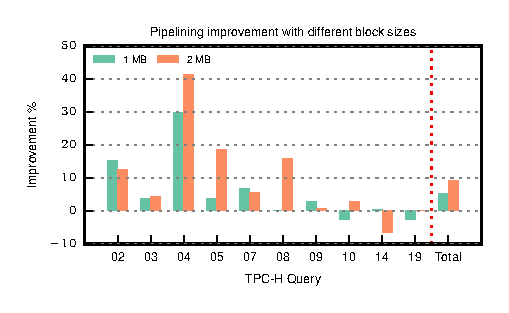
\includegraphics[width=0.6\textheight]{pipeline/figures/tpch-ccs-block-size-ratio}
	\caption{Impact of block size on query performance improvement due to pipelining}
	\label{fig:tpch-ccs-block-size-ratio}
\end{figure}

We observe that w.r.t total execution time, the improvement due to pipelining in both block sizes is not very significant (10\%).

TPC-H Q04 pipelining strategy benefits significantly from 2 MB block sizes.
As explained earlier in Section~\ref{ssec:overall-execution-time}, the build operator in Q04 has issues with scalability. 
A 2 MB block size helps alleviate the scaling issues; as larger block size implies fewer work orders for the build hash table operator. 
We present the mean work order execution times of the two dominant operators in TPC-H Q04 in Figure~\ref{fig:tpch-q04-ccs-mean-wo-times}.
We can observe that the gap between build operators' execution time for 2 MB non-pipelining version and 2 MB pipelining version is higher than the 1 MB counter part. 

\begin{figure}
	\centering 
	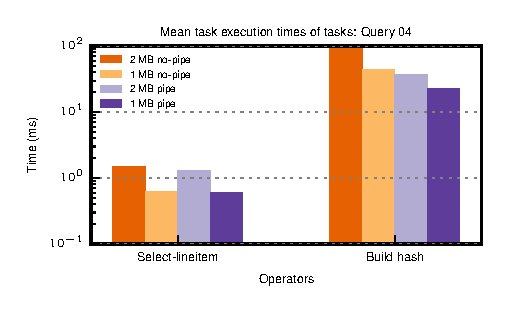
\includegraphics[width=0.6\textheight]{pipeline/figures/tpch-q04-ccs-block-size-mean-wo-times}
	\caption{Mean work order execution times of dominant operators in TPC-H Q04}
	\label{fig:tpch-q04-ccs-mean-wo-times}
\end{figure}

\subsubsection{Effect of Storage Format}
Next we study the effect of storage format of base tables on the pipelining performance. 
We use two configurations: a) All TPC-H tables stored in row store format b) All TPC-H tables stored in column store format. 
Then we compare the improvement of pipelining over non-pipelining for each configuration. 
Note that in both configurations, temporary tables are stored in row store format. 
We run the queries using 20 threads and block size of 2 MB.

\begin{figure}
	\centering 
	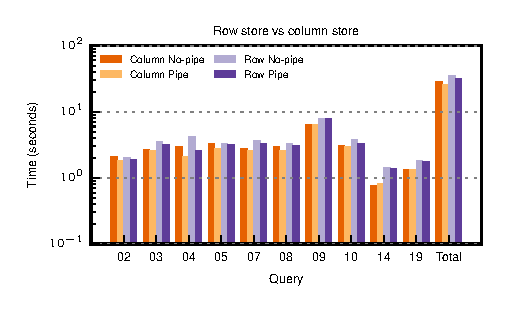
\includegraphics[width=0.6\textheight]{pipeline/figures/tpch-rowstore-vs-ccs-total-time-absolute}
	\caption{Comparison of pipelining vs non-pipelining for row store and column store storage formats}
	\label{fig:tpch-rowstore-vs-ccs-total-time-absolute}
\end{figure}

First, we can observe that column store queries are slightly faster than their row store counterparts. 
Second, the total query execution time is not significantly different between using pipelining and non-pipelining strategy. 
\todo{Write conclusions}

\subsubsection{Effect of number of threads}
Next, we study the effect of number of threads on the performance of pipelining and non-pipelining strategies. 
In each experiment, we set the number of worker threads in \sys{} to a given value (10 and 20).
Figure~\ref{fig:tpch-thread-effect-ccs} shows the comparison between pipelining and non-pipelining strategies when the number of threads are varied. 

Notice that using 10 threads, the query performances are identical in pipelining and non-pipelining implementation. 
The reasons are as follows:
 As the number of threads decrease, effective degree of parallelism for operators decrease. 
We observed earlier that pipelining implementation gained performance due to scalability limitations of operators.
With fewer threads, the amount of this gain comes down.
Moreover with fewer threads it takes more time for output to be ready for a consumer operator in a pipeline.
Therefore pipelining implementation starts to behave more like non-pipelining implementation.  

\begin{figure}
	\centering 
	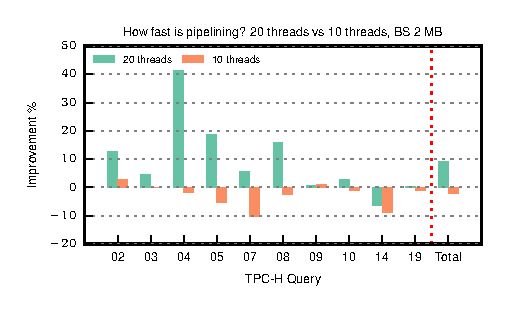
\includegraphics[width=0.6\textheight]{pipeline/figures/thread-effect-ccs-bs2mb}
	\caption{Comparison of pipelining vs non-pipelining for varying number of threads}
	\label{fig:tpch-thread-effect-ccs}
\end{figure}

\subsubsection{Effect of prefetching}
We examine the effect of prefetching on the relative performance of pipelining and non-pipelining implementation. 
We run the queries using pipelining and non-pipelining strategies in two scenarios: a) hardware prefetching is enabled b) hardware prefetching is disabled (by setting bit 0 and 1 in MSR 0x1A4 ~\cite{intel-prefetching}).

First, let us look at the role played by prefetching on individual strategies.
Figure~\ref{fig:prefetching-vs-noprefetching-ccs} presents the improvements in query execution times due to hardware prefetching. 

\begin{figure}
	\centering 
	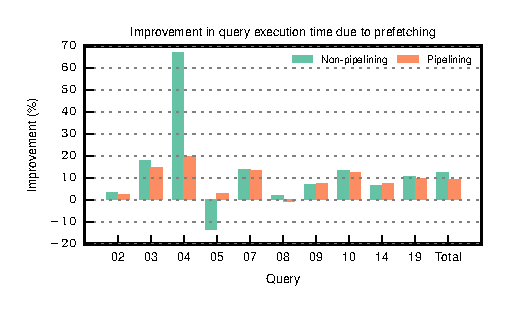
\includegraphics[width=0.6\textheight]{pipeline/figures/prefetching-improvement-tpch-ccs-20threads-bs2mb}
	\caption{Benefit of hardware prefetching on individual strategies in column store}
	\label{fig:prefetching-vs-noprefetching-ccs}
\end{figure}

Figure~\ref{fig:prefetching-vs-noprefetching-ccs} shows the benefits of prefetching on pipelining and non-pipelining strategies.
Note that prefetching does not benefit many queries (except Q04) and the overall execution time.
However a similar analysis on the rowstore shows that prefetching enables big improvements for many queries, as shown in Figure~\ref{fig:prefetching-vs-noprefetching-rowstore}. 

The gains shown for prefetching are higher for rowstore are higher than that for column store. 
In the row store format, even if a single attribute is scanned, a lot of unnecessary data from the tuple is read.
As rowstore tuples are fixed width\footnote{variable length attributes are stored in a separate region, with a pointer to the region stored in the tuple}, the hardware prefetcher can detect the access pattern of scanning a single attribute. 
Contrast to column store where values from an attribute are located in a contiguous region, thus scanning an attribute does not involve reading unnecessary data. 
Therefore the prefetcher does not make any significant contribution to an already optimized access pattern.
Hence the gains by prefetching are higher for rowstore. 
\begin{figure}
	\centering 
	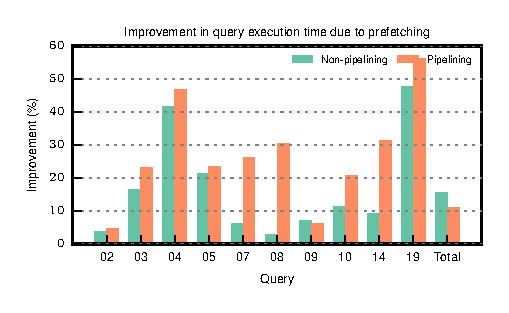
\includegraphics[width=0.6\textheight]{pipeline/figures/prefetching-improvement-tpch-rowstore-20threads-bs2mb}
	\caption{Benefit of hardware prefetching on individual strategies on row store}
	\label{fig:prefetching-vs-noprefetching-rowstore}
\end{figure}

Next we take a look at effects of prefetching on operator task execution times. 
Selection operation is more amenable to hardware prefetching, due to its sequential access pattern, therefore we focus only on the selection operation. 
We pick TPC-H Q19 from rowstore, as it benefits the most among the observed queries.	
Figure~\ref{fig:tpch-q19-prefetching-benefits-selectionwo}, presents the improvements caused by prefetching on mean selection operator task execution time. 

\begin{figure}
	\centering 
	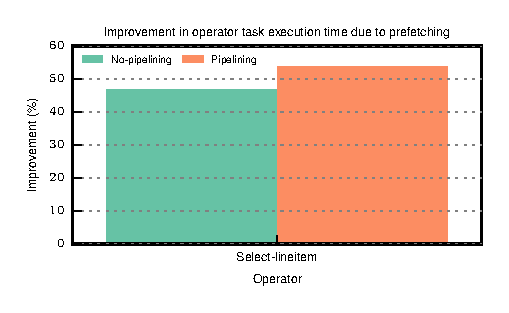
\includegraphics[width=0.6\textheight]{pipeline/figures/tpch-q19-rowstore-prefetching-benefits-selectionwo}
	\caption{Impact of prefetching on the selection operator task's performance for TPC-H Q19 with rowstore}
	\label{fig:tpch-q19-prefetching-benefits-selectionwo}
\end{figure}

We can observe that the selection operator's performance in both strategies benefit from prefetching. 
As the selection operator is the dominant operator in TPC-H Q19, the benefits of prefetching for selection operator translate to benefit in total query execution time. 

\subsection{Evaluation of Pipeline Sequencing Algorithm}
We now evaluate the effect of our pipeline sequencing algorithm proposed in Section~\ref{sec:pipe-seq-algo}.

\begin{figure}[t]
	\centering
	\begin{subfigure}[b]{0.45\textwidth}
		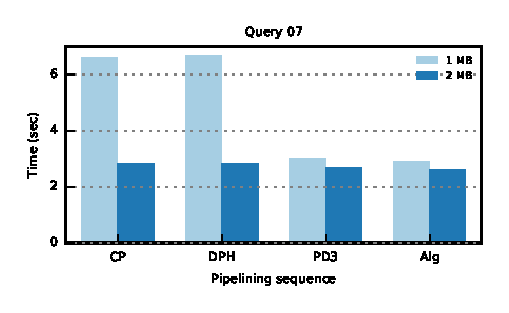
\includegraphics[width=\textwidth]{pipeline/figures/sequence-analysis-q07-bs1mb-bs2mb.pdf}
		\caption{Q07}
	\end{subfigure} %
	~
	\begin{subfigure}[b]{0.45\textwidth}
		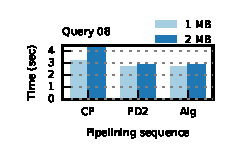
\includegraphics[width=\textwidth]{pipeline/figures/sequence-analysis-q08-bs1mb-bs2mb.pdf}
	\caption{Q08}
	\end{subfigure}%
	\caption{Evaluation of the pipeline sequencing algorithm on block size 1 MB and 2 MB}
	\label{fig:pipeline-sequence-results}
\end{figure}

We use two TPC-H queries Q07 and Q08 because their query plan is complex enough so that we can produce multiple pipeline sequences and compare them against the output of our pipeline sequencing algorithm.
We run the experiment with two block sizes viz 1 MB and 2 MB stored in the column store format.
We use all the 20 threads on the socket to run the queries.

We acknowledge that there can be large number of pipeline sequences possible for each query plan. 
To keep our analysis focused, we pick representative sequences whose behavior can be easily explained.
The sequence CP denotes the sequence in which the probe input is cold, but the hash table is hot just before the beginning of the probe operation. 
The sequence DPH indicates that the dominant selection-probe pipeline is hot, thereby majority of the probe operations are served from hot input. 
The sequence PD$N$ denotes that the maximum depth of the pipeline is $N$. 
We set the N such that it is one less than the depth of the longest pipeline output by our algorithm.
Finally, Alg denotes the sequence output by our algorithm.

Figure~\ref{fig:pipeline-sequence-results} presents the results for this evaluation.
We note that the sequence output by our algorithm almost always results in the lowest execution time. 

The cold probe sequences perform the worst both in Q07 and Q08, underscoring the importance of hot probe input. 

The DPH sequence in Query 07 results in poor performance, because there is scalability issue with a certain probe operator in the query plan that has to probe a big hash table built on the entire orders table.
The reconstruction of output tuples require accessing large orders table, and thus higher concurrency implies large random read traffic. 
Therefore the probe operator can't scale with increasing number of threads, thus it should have a lower DOP.
In the sequence output by our algorithm, and PD3 this probe operator is at the middle of the pipeline.
Hence naturally the DOP of this operator is low, hence these two sequences perform well.

We also note that PD$N$ sequences perform similarly to our algorithm, due to the low amount of work at the end of the pipeline.